% !TeX spellcheck = en_US

\documentclass[12pt]{beamer}
\usepackage{pgfkeys}
\usepackage{pgfopts}
\usetheme[color/background=white]{emc}
\usepackage[utf8]{inputenc}
\usepackage{amsmath}
\usepackage{amsfonts}
\usepackage{amssymb}
\usepackage{nicefrac}
\usepackage{graphicx}
\usepackage{subcaption}
\usepackage{fancyvrb}
\usepackage{wasysym}
%\usepackage{minted}
\usepackage{listings}
\usepackage{gitdags}
\usepackage{textcomp}

\usepackage{tikz}
\usetikzlibrary{shapes, arrows, calc}


\lstset{basicstyle=\ttfamily,
	showstringspaces=false,
	commentstyle=\color{red},
	keywordstyle=\color{blue}
}
\author{Sten Willemsen}
\title{Using GIT}

\begin{document}
\begin{frame}
	\titlepage
\end{frame}


\begin{frame}{Table of contents}
  \setbeamertemplate{section in toc}[sections numbered]
\end{frame}

\section{Introduction}

\begin{frame}{Why GIT}
	\begin{itemize}
	\item Hi Sten. Which file should I look at to see the changes you made last week?
	\item O, you also need to work with the newest version of utilfuncs.R in order for that program to work
	\item What has changed between November and now
	\item Can you send me the version that was submitted to Statistical Modelling
	\end{itemize}
\end{frame}

\begin{frame}[fragile]{Why GIT}
	\begin{itemize}
	\item Sometimes versioning is done by using some naming scheme. 
	\end{itemize}
	\begin{lstlisting}[language=bash, escapeinside={<@}{@>}]
	analysis.sps
	analysis1.sps
	analysisFinal.sps
	analysisFinal_long.sps
	analysisFinal_revision.sps
	analysisFinal_revisionnew.sps
	analysis2.sps
	\end{lstlisting}
\begin{itemize}
\item 	However it is not always clear to other people
\item 	And probably not even to your future self
\end{itemize}
\end{frame}

\begin{frame}{Why GIT}
	\begin{itemize}
	\item  `Version control systems' (VCSs)are pieces of software that help you manage different versions of programs (documents etc ldots)
	\begin{itemize}
		 \item Easy to go back to older versions
		 \item Assist in maintaining multiple versions in parallel (e.g. windows / linux)
		\item simplifies working in teams
		\end{itemize}
	\item There are different `version control systems' (VCSs)
		\begin{itemize}
		\item CVS, Subversion, Bazaar, Mercurial, Perforce, Git
		\end{itemize}
	\item We can distinguish between:
	\begin{itemize}
		\item systems with a central repository (cvs, subversion) and
		\item systems where all repositories are treated as equal (Mercurial Git)
		\end{itemize}
	  	
	\end{itemize}
	
\end{frame}

\begin{frame}{Why GIT}
	\begin{itemize}	
      \item It seems that now git is more or less the standard	
	\end{itemize}
	\begin{center}
	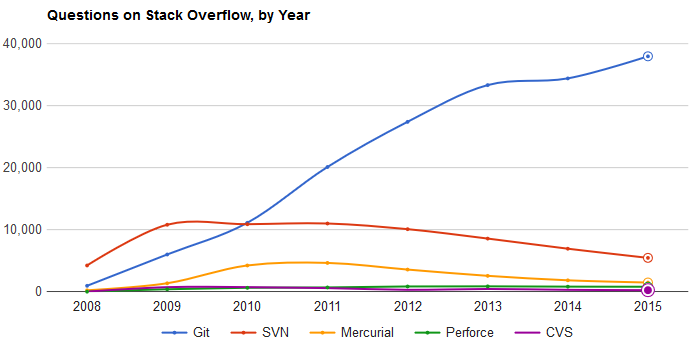
\includegraphics[width=\linewidth]{NumberOfQuestions}
	\end{center}
	{\tiny source: https://rhodecode.com/}
\end{frame}

\section{Git basics}

\begin{frame}{Why GIT}
	\begin{itemize}	
      \item Git primarily works via the command line
      \item When you install git for windows an environment is created that includes some of the basic tools that are also available on linux/unix machine including a version \alert{bash}
      \item There are a number of GUIs (which I personally do not like that much)
      \item Git is also supported from a number of other software packages 
	\end{itemize}
\end{frame}



\begin{frame}[fragile]{Starting a project}
\begin{itemize}
\item To start a git project in an existing directory:
\end{itemize}
\begin{lstlisting}[language=bash, escapeinside={<@}{@>}]
git init
\end{lstlisting}
\begin{itemize}
	\item A \attention{.git} folder will be added that contains the information git needs
\end{itemize}
\begin{itemize}
\item Files can be added with:
\end{itemize}
\begin{lstlisting}[language=bash, escapeinside={<@}{@>}]
git add myexamplefile.txt
\end{lstlisting}
\end{frame}

\begin{frame}[fragile]{Cloning from a server}
\begin{itemize}
\item To get a copy from a project that is located on a remote repository (like github or bitbucket):
\end{itemize}
\begin{lstlisting}[language=bash, escapeinside={<@}{@>}]
git clone \
  https://github.com/stenw/emcbeamertheme.git
\end{lstlisting}
\begin{itemize}
\item The files are now copied to your \textbf{\attention{working directory}}
\end{itemize}
\end{frame}


\begin{frame}[fragile]{Basic work flow}
\begin{itemize}
\item Committing changes in git is a two step process 
\item You can mark the files for which you want to commit the changes using \texttt{git add}. Files are now put in the \textbf{\attention{staging area}} or \textbf{\attention{index}}
\item changes can be committed using \texttt{git commit}
\item So after making a change to the file myexamplefile.txt we do:
\end{itemize}
\begin{lstlisting}[language=bash, escapeinside={<@}{@>}]
git add myexamplefile.txt
git commit
\end{lstlisting}
\begin{itemize}
\item This opens your editor so you can write a commit message
\end{itemize}
\end{frame}


\begin{frame}[fragile]{Basic work flow}
\begin{itemize}
\item When you use \texttt{git commit} git creates a commit object  
\item This represents the current state of your project
\item The commit object is (usually) based on a previous commit (the parent)
\item Usuall a commit has a single parent but by \textbf{\attention{merging}} (discussed later) we can create commits that have multiple parents
\item The commits form a DAG
\item The `active' commit is called the \textbf{\texttt{HEAD}}
\end{itemize}

\begin{figure}

    \centering
    \begin{tikzpicture}
      % Commit DAG
      \gitDAG[grow right sep = 2em]{
        A -- B -- C,
      };
      % Tag reference
           % Branch
       % target
      % HEAD reference
      \gitHEAD
        {above=of C} % node placement
        {C}          % target
    \end{tikzpicture}



  \caption{Simple linear development}
\end{figure}
\end{frame}

\begin{frame}[fragile]{Basic work flow}
	\begin{itemize}
		\item \texttt{git log} Shows you the commit history 
		\item \texttt{git checkout <commit>} let's you go back to an old commit
		\item The argument to this function is the SHA-1 hash that uniquely defines the commit
	\end{itemize}
\end{frame}


\begin{frame}[fragile]{Basic work flow}
\begin{itemize}
\item \texttt{git status} lets you see which files
\begin{itemize}
\item are under version control
\item have changes
\item are staged for commit
\end{itemize}
\item \texttt{git diff} shows you differences
\begin{itemize}
\item \texttt{git diff}: differences between working directory and index
\item \texttt{git diff --staged}: differences between index and HEAD 
\item \texttt{git diff HEAD}:  differences between your working directory and HEAD
\item We can also compare with an other commits or compare commits with each other
\end{itemize}

\end{itemize}
\end{frame}

\begin{frame}[fragile]{Basic work flow}
	\def\blockdist{2.3cm}
	\begin{tikzpicture}
	\node (A) [text width=\blockdist, draw, fill= emclblue!20, minimum height=2cm, minimum width=5cm] {\Large HEAD};
	\path (A.0)+(0,-2*\blockdist) node (WD)[rectangle, draw, fill= emclblue!20, text width=\blockdist,  minimum width=6cm] {\large Working Directory};
	\path (A.180)+(0,-\blockdist) node (I)[rectangle, draw, fill= emclblue!20, text width= 3cm, minimum width=6cm] {\large Index};
	\coordinate (aid1) at (A.south);
	\coordinate (aid2) at (I.south);
	\coordinate (aid3) at (WD.north);
	\coordinate (aid4) at (aid1 |- aid2) ;
	\coordinate (aid5) at (aid1 |- aid3) ;
	\draw [->, ultra thick] (A.south east) -- (WD) node [pos=0.5, right] (lab1) {git diff --HEAD};
	\draw [->, ultra thick] (A.south west) -- (I) node [pos=0.5, left] (lab2) {git diff --staged};
	\draw [->, ultra thick] (aid4) -- (aid5) node [pos=0.5, left] (lab3) {git diff };	
	\end{tikzpicture}
\end{frame}


 \section{Branches and merging}

\begin{frame}[fragile]{Branches}
\begin{itemize}
\item A Branch represents an independent (parallel) line of development
\item This is useful when we want to introduce multiple versions of a program
\item Also used when working on a new feature
\begin{itemize}
\item In this way you can work on multiple things at the same time without breaking it (for other people)
\end{itemize}
\item \texttt{git branch} lists all branches
\item \texttt{git branch <branchname>} creates a new branch
\item \texttt{git checkout <branchname>} switch to branch
\item The last commit in a branch is called the \textbf{\attention{tip}}
\item The `main' development branch is by conventionally called \attention{master}
\end{itemize}

\end{frame}

\begin{frame}
	\begin{figure}
 \begin{tikzpicture}
 \gitDAG[grow right sep = 2em]{
        A -- B -- { 
          C -- D,
          E -- F -- G,
        }
      };
      % Branch
      \gitbranch
        {master}     % node name and text 
        {above=of D} % node placement
        {D}          % target
      \gitbranch
              {develop}     % node name and text 
              {above=of G} % node placement
              {G}     
      % HEAD reference
      \gitHEAD
        {above=of master} % node placement
        {master}          % target
    \end{tikzpicture}
     \caption{Example with branches}
\end{figure}
\end{frame}

\begin{frame}[fragile]{Merging}
\begin{itemize}
\item Different branches can be put together again using a \textbf{\attention{merge}}
\item \texttt{git merge <branch>} merges $\langle$branch$\rangle$ into the current branch
\item Depending on the state of the branches git will determine the kind of merge that will be performed
\item Fast-forward merge occurs by just moving the tip of the branch. This is the most simple kind of merge.
\end{itemize}
\end{frame}



\begin{frame}{fast-forward merge}
	 \begin{figure}
 \begin{subfigure}[b]{\textwidth}
	\centering
	\begin{tikzpicture}
	% Commit DAG
	\gitDAG[grow right sep = 1em]{
		A -- B -- C -- D -- E,
	};
	% Tag reference
	% Branch
	\gitbranch
	{master}     % node name and text 
	{above=of C} % node placement
	{C}          % target
	\gitbranch
	{devel}     % node name and text 
	{above=of E} % node placement
	{E}    
	% HEAD reference
	\gitHEAD
	{above=of master} % node placement
	{master}          % target
	\end{tikzpicture}
\subcaption{before}
\end{subfigure}
\\[3pt]
\begin{subfigure}[b]{\textwidth}
	\centering
	\begin{tikzpicture}
	\gitDAG[grow right sep = 1em]{
	A -- B -- C -- D -- E,
};
% Tag reference
% Branch
\gitbranch
{devel}     % node name and text 
{above=of E} % node placement
{E}          % target
\gitbranch
{master}     % node name and text 
{above=of devel} % node placement
{devel}    
% HEAD reference
\gitHEAD
{above=of master} % node placement
{master}          % target
	\end{tikzpicture}
	\subcaption{after}
\end{subfigure}
\end{figure}
\end{frame}

\begin{frame}[fragile]{Merging}
	\begin{itemize}
		\item Often fast-forward merge is not possible and a separate commit has to be used to combine the histories
		\item When the two branches have modified the same part of a file git does not know which change to accept. This is called a \textbf{\attention{merge conflict}}. You have to resolve this conflict yourself. 
	\end{itemize}
\end{frame}

\begin{frame}
\begin{tikzpicture}
\tikzstyle{commit} = [fill=blue!20, circle]
\node (S1) [draw, DAGcommit, label=left:{Initial commit}] {};
\node (S2) [below=of S1,   DAGcommit, label=left:{Sten does some work}] {};
\node (S3) [below=of S2, DAGcommit, label=left:{\begin{tabular}{r} Sten implements \\ a cool feature\end{tabular}}] {};
\node (S4) [below=of S3, DAGcommit, label=left:{Merge}] {};
\node (C1) [below right=of S2, DAGcommit, label=right:{\begin{tabular}{l}Cibele corrects \\  mistake \end{tabular}}] {};
\draw [DAGedge] (S1) -- (S2) ;
\draw [DAGedge] (S2) -- (S3) ;
\draw [DAGedge] (S3) -- (S4) ;
\draw [DAGedge] (S2) -- (C1) ;
\draw [DAGedge] (C1) -- (S4) ;
\end{tikzpicture}
\end{frame}

\begin{frame}[fragile]{Manually merging}
		\begin{itemize}
			\item You can mopen up an editor and deal with all conflicts
		\end{itemize}
	\begin{lstlisting}[language=bash, escapeinside={<@}{@>}]
	<@\textcolor{blue}{ 
	<<<<<<< HEAD:lyrics.txt
	\\
	doo-bi-doo-bi-doo
	}@> 
	=======
	<@\textcolor{red}{ 
	doo-ba-doo-ba-doo 
	\\
	>>>>>>> develop:lyrics.txt 
	}@>
	\end{lstlisting}
		\begin{itemize}
		\item There are also tools to help you with this (I like meld). \texttt{git mergetool} can be configured to start these programs to resolve all conflicts.
		\end{itemize}
\end{frame}

\begin{frame}[fragile]{Rebase}
	\begin{itemize}
		\item \texttt{\attention{git rebase}} forms an alternative to merge
		\item It applies changes made in a branch and applies them to an other branch
	\end{itemize}
 \begin{alertblock}{Warning}
	\textbf{Rebase} changes your history so use with care
\end{alertblock}

\end{frame}

\begin{frame}[fragile]{Rebase}
\begin{figure}
		\centering
		\begin{tikzpicture}
		% Commit DAG
		\gitDAG[grow right sep = 2em]{
			A -- B -- { 
				C,
				D -- E,
			}
		};
		% Tag reference
		% Branch
		\gitbranch
		{feature}     % node name and text 
		{above=of E} % node placement
		{E}          % target
		\gitbranch
		{master}     % node name and text 
		{above=of C} % node placement
		{C}          % target
		% HEAD reference
		\gitHEAD
		{above=of master} % node placement
		{master}          % target
		\end{tikzpicture}
		\caption{Before\ldots}

	\end{figure}
\end{frame}

\begin{frame}{Rebase}
\begin{figure}
	\centering
	\begin{tikzpicture}
	% Commit DAG
	\gitDAG[grow right sep = 2em]{
	 A -- B -- { 
		C -- D' -- E',
		{[nodes=unreachable] D -- E },
	}
};
	% Tag reference
	% Branch
	\gitbranch
	{feature}     % node name and text 
	{above=of E'} % node placement
	{E'}          % target
	\gitbranch
	{master}     % node name and text 
	{above=of C} % node placement
	{C}          % target
	% HEAD reference
	\gitHEAD
	{above=of master} % node placement
	{master}          % target
	\end{tikzpicture}
	\caption{\ldots and after}
	
\end{figure}
\end{frame}


\section{Remote branches}

\begin{frame}[fragile]{Working with a remote repository}
\begin{itemize}
\item Often we want to work with a server
\item We can get the new commits from the server using \texttt{git fetch}
\item These changes can now be merged with the local branches
\item We can combine the fetch with the merge using \texttt{git pull}
\item Local commits can be moved to the server using \texttt{git push}
\end{itemize}
\end{frame}


\section{Other commands}

\begin{frame}{Git diff}
	Different types of diff
	\begin{itemize}
    \item git diff: Show differences between your working directory and the index.
    \item git diff –cached: Show differences between the index and the most recent commit.
    \item git apply: Go back to a stored state
	\end{itemize}	
\end{frame}	

\section{Other commands}

\begin{frame}{Git stash}
	\begin{itemize}
		\item \textbf{\texttt{git stash}}: Stores state of working directory and then go back to a clean state
		\item \textbf{\texttt{git stash list}}: Show stored states
		\item \textbf{\texttt{git stash apply}}: Go back to a stored state
	\end{itemize}	
\end{frame}	

\begin{frame}{Git reset}
	\begin{itemize}
		\item \textbf{\texttt{git reset --soft <commit>}}: Moves HEAD to another commit
		\item \textbf{\texttt{git reset --mixed <commit>}}: Moves HEAD to another commit and updates the index (to new HEAD) (this is the default)
		\item \textbf{\texttt{git reset --hard <commit>}}: Like the previous but also resets the working directory
	\end{itemize}	
\end{frame}	

\begin{frame}{Git rm}
	\begin{itemize}
		\item \textbf{\texttt{git rm  <file>}}: removes a file from the working directory and the index (it is no longer under version control)
		\item \textbf{\texttt{git rm <file>}}: Stage file for deletion but keep in working directory
	\end{itemize}	
\end{frame}	

\section{Discussion points}

\begin{frame}{Points for discussion}
	\begin{itemize}
		\item Git does not play along nicely with latex paragraphs
		\item Hard to make single topic commits with clear commit messages
		\item Should results be kept (what if the computations take a long time)
		\item What about the input / data files
		\item Different variants of a program within a branch?
		\item What to do with MS Word files etc
		\item Should we think about a standard work-flow?
		\item Do we need our own git server
		\item ... 
	\end{itemize}	
\end{frame}	

\end{document}
